\section{Material Design}
Material Design ist eine Design Sprache (Design Language). Eine Design Sprache ist eine Hilfestellung für den Designprozess. Es beschreibt, wie die Teile einer Applikation aussehen und sich verhalten sollen. Material ist die Metapher und arbeitet im 3D-Raum mit Licht und Schatten. Es ist angelehnt an physikalische Begebenheiten. Man verwendet ein Grid für die Ausrichtung und versucht, wenn angemessen eine Reaktion auf User-Input zu geben. Materials sind geometrische Formen (Schnipsel aus Papier) mit einer Dicke von exakt 1dp. Duch die unterschiedliche Anordnung auf der Z-Achse entsteht Schatten. Dieses Konzept hat Einfluss auf verschiedene Aspekte. Material Design Styleguides umfasset deshalb auch: Layout, Style, Animation, Components, Patterns und Usability.\\
\paragraph{Layout} Grundelement ist das Papier, das an- und übereinander gelegt werden kann. Ein Floating Action Button beispielsweise, bietet eine Aktionsmöglichkeit für das Papier. Alle anderen Materialien werden an einem 8dp Grid ausgerichtet.
\paragraph{Layout Spacing} Der Abstand zwischen Elementen ist meist ein Vielfaches von 8. \\
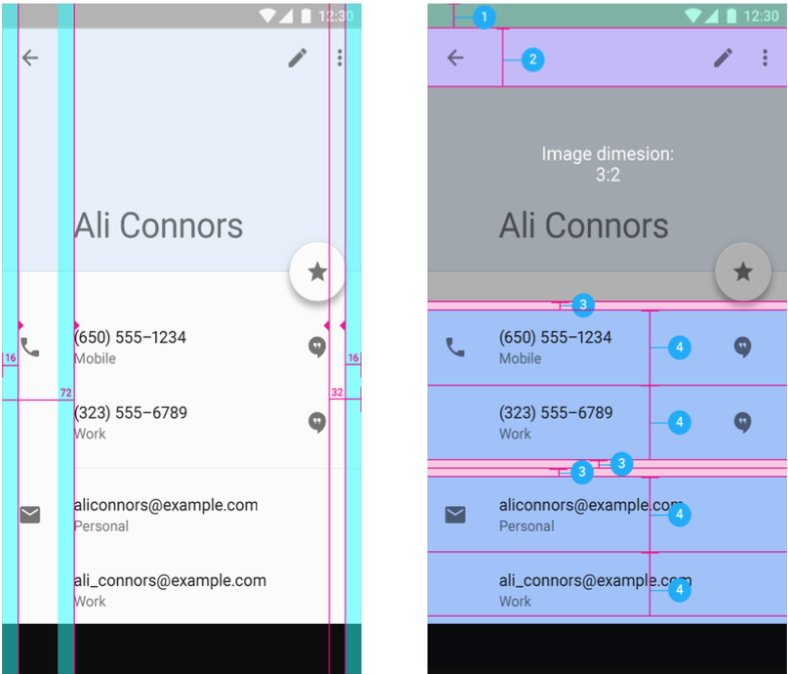
\includegraphics[scale=0.25]{LayoutSpacing.png}
\begin{enumerate}
\item Status bar: 24dp
\item Toolbar: 56dp
\item Space: 8dp
\item List item: 72dp
\end{enumerate}
\paragraph{Style} Für Material Design wird empfohlen, dass man 3 Farbtöne der Primärpalette und eine Akzentfarbe aus einer zweiten Palette wählt. 
\paragraph{Animation} helfen die Illusion aufrecht zu halten, dass wir die Materialien auf dem Screen direkt manipulieren (wie durch eine Glasscheibe). Man sollte visuelles Feedback auf Input geben und den Übergang zwischen Zuständen animieren. 
\paragraph{Usability} Wichtige Punkte in Usability sind:
\begin{itemize}
\item Touch-Targes nicht zu klein machen
\item Navigation soll nachvollziehbar und nicht komplex sein
\item Fontgrössen, Farben
\item RTL-Layouts werden (wenn richtig gemacht automatisch) gespiegelt
\item Texte in Grafiken sind problematisch
\end{itemize}
\subsection{Umsetzung}
\paragraph{View Styling} Views können direkt im XML-Layout gestyled werden. 
\begin{lstlisting}[language=xml]
<Button
  android:layout_width="wrap_content"
  android:layout_height="wrap_content"
  android:text="New Button"
  android:id="@+id/button2"
  android:layout_gravity="center"
  android:background="#ff85e1"
  android:height="36dp"
  android:minWidth="64dp"
  android:padding="8dp" />
\end{lstlisting}
Meist ist es am schönsten wenn man so etwas in ein Style auslagert.
\begin{lstlisting}[language=xml]
<style name="MyButtonStyle">
  <item name="android:background">#ff85e1</item>
  <item name="android:height">36dp</item>
  <item name="android:minWidth">64dp</item>
  <item name="android:padding">8dp</item>
</style>
\end{lstlisting}
Dies wird dann mit \code{style="@style/MyButtonStyle"} referenziert. Auch diese Ressourcen können für unterschiedliche Geräte, Versionen etc. spezifiziert werden. 
\paragraph{Themes} sind Styledefinitionen die für eine Activity oder App gelten
\begin{lstlisting}[language=xml]
<application
  ...
  android:theme="@style/AppTheme">
  <activity
  android:name".MainActivity"
  android:theme="@style/AppTheme" >
\end{lstlisting}
Das AppTheme ist das Standarttheme, und müsste nicht spezifiziert werden. Im \code{styles.xml} kann man die entsprechenden Styles definieren.
\begin{lstlisting}[language=xml]
<style name="AppTheme" parents="Theme.AppCompat.Light.NoActionBar">
<!-- Ueberschreiben von Theme einstellungen -->
</style>
\end{lstlisting}
Im Theme definierte Styles können in anderen Ressourcen referenziert werden, anstelle eines \@ wird ein ? verwendet. Bei der Syntax gibt es zwei Varianten:
\begin{lstlisting}[language=xml]
<!-- colorAccent ist im Theme definiert -->
<style name="AccentedButton">
  item name="android:background">?colorAccent
</style>
<Button android:background="?attr/colorAccent" />
<!-- gleich wie -->
<Button android:background="?/colorAccent" />
\end{lstlisting}


Die Aktzenfraben können im Style.xml definiert werden
\begin{lstlisting}[language=xml]
<item name="primary" type="color">#3F51B5</item>
<item name="primary_dark" type="color">#303F9F</item>
<item name="accent" type="color">#FF4081</item>
\end{lstlisting}
\paragraph{Theme Overlays} Die Kombination von Light-Theme und dunkler Toolbar führt dazu, dass die Schrift in der Toolbar schwarz ist. View können keine eigenen Themes haben, aber Theme Overlays, die einen Teil der Theme-Attribute überschreiben.
\begin{lstlisting}[language=xml]
<android.support.v7.widget.Toolbar
  ...
  app:theme="@style/ThemeOverlay.AppCompat.Dark.ActionBar"
  app.popupTheme="@style/ThemeOverlay.AppCompat.Light" />
\end{lstlisting}
\paragraph{Floating Action Button} Der FAB bietet eine primäre Aktion für die darunterliegende View an.
\begin{lstlisting}[language=xml]
<android.support.design.widget.FloatingActionButton
  android:src="@drawable/plus"
  android:onClick="onPlusClicked" />
\end{lstlisting}
\paragraph{TextInputLayout} Dies ist ein EditText, bei dem der Hinweistext beim editieren nicht verschwindet.
\begin{lstlisting}[language=xml]
<android.support.design.widget.TextInputLayout
  android:id="@+id/username_text_input_layout"
  android:layout_width="match_parent"
  android:layout_height="wrap_content
  android:layout_gravity="center" >
  <EditText
  android:id="@+id/username_edit_text"
  android:layout_width="match_parent"
  android:layout_height="wrap_content"
  android:hint="Your username"
  android:layout_gravity="center" />
</android.support.design.widget.TextInputLayout>
\end{lstlisting}
\paragraph{Scrollende Toolbar} Die Toolbar kann auch mit dem Inhalt weggescrollt werden. 
\begin{lstlisting}[language=xml]
<android.support.design.widget.CoordinatorLayout xmlns:android="..." xmlns:app="..."
  android:layout_width="match_parent" android:layout_height="match_parent">
  <android.support.v7.widget.RecyclerView
  android:id="@+id/recyclerView"
  android:layout_width="match_parent"
  android:layout_height="match_parent"
  app:layout_behavior="@string/appbar_scrolling_view_behavior" />
  <android.support.design.widget.AppBarLayout
  android:id="@+id/appBarLayout"
  android:layout_width="match_parent"
  android:layout_height="wrap_content">
  <android.support.v7.widget.Toolbar
  android:id="@+id/toolbar"
  android:layout_width="match_parent"
  android:layout_height="?attr/actionBarSize"
  app:layout_scrollFlags="scroll|enterAlways"/>
</..>
\end{lstlisting}
\paragraph{Zusammenklappbare Toolbars} Toolbars die Verschwinden können.
\begin{lstlisting}[language=java]
<android.support.design.widget.AppBarLayout
  ...
  android:layout_height="128dp">
  <android.support.design.widget.CollapsingToolbarLayout
  android:id="@+id/collapsing_toolbar"
  android:layout_width="match_parent"
  android:layout_height="match_parent"
  app:contentScrim="?attr/colorPrimary"
  app:expandedTitleMarginEnd="64dp"
  app:expandedTitleMarginStart="48dp"
  app:layout_scrollFlags="scroll|exitUntilCollapsed">
  <android.support.v7.widget.Toolbar
  android:id="@+id/toolbar"
  android:layout_width="match_parent"
  android:layout_height="?attr/actionBarSize"
  app:layout_collapseMode="pin" />
\end{lstlisting}
\paragraph{Tab Navigation} Dies ist kein neues Feature, aber mit dem CoordinatorLayout und AppBarLayout integriert worden. Tabs sind unterschiedliche Screens (Fragments), und Swipe oder Touch wechselt zwischen Tabs.
\begin{lstlisting}[language=xml]
<CoordinatorLayout>
  <AppBarLayout>
  <Toolbar />
  <TabLayout />
  </AppBarLayout>
  <ViewPager />
</CoordinatorLayout>
\end{lstlisting}
Das TabLayout zeigt die Liste der Tabs an, der ViewPager den Inhalt der Tabs (wechselt zwischen Fragments).
\begin{lstlisting}[language=java]
@Override
protected void onCreate(Bundle savedInstanceState) {
  ...
  ViewPager vp = (...)findViewById(R.di.viewpager);
  ViewPagerAdapger adapter = new ViewPagerAdapger(getSupportFragmentManager());
  adapter.addFragment(new ListFragment(), "CALLS");
  adapter.addFragment(new ListFragment(), "CHATS");
  adapter.addFragment(new ListFragment(); "CONTACTS");
  vp.setAdapter(adapter);
  TabLayout tl = (...)findViewById(R.id.tabs);
  tl.setupWithViewPager(vp);
\end{lstlisting}
Diese Toolbar lässt sich beim Scrollen auch verstecken.
\begin{lstlisting}[language=java]
<android.support.design.widget.CoordinatorLayout ...>
  <android.support.design.widget.AppBarLayout ...>
  <android.support.v7.widget.Toolbar ...
    app:layout_scrollFlags="scroll|enterAlways />
  <android.support.design.widget.TabLayout .../>
  </android.support.design.widget.AppBarLayout>
  <android.support.v4.view.ViewPager ..
  app:layout_behavior="@string/appbar_scrolling_view_behavior" />
</android.support.design.widget.CoordinatorLayout>
\end{lstlisting}
Dies klappt jedoch nur, wenn die Fragments RecylcerView oder NestedScrollViews sind (nicht mit ListViews oder ScrollViews).
